\hfill \break
\subsection*{Algoritmo Partition}
    La función clave en QuickSort es Partition(). El objetivo de esta función es, dado un arreglo toma como "pivote" al ultimo elemento del arreglo y pone al elemento tomado como pivote en la posición correcta del arreglo. Pone a los elementos menores al pivote a su izquierda y aquellos mayores a su derecha.
    
    El pseudocódigo  del algoritmo se muestra en la figura \ref{PseudocodigoPartition}:
    
    \begin{figure}[h!]
        \centering
        \begin{verbatim}
            int Partition(int A[], int prim, int ult)
                int pivote = A[ult]
                int i=prim-1
                for j=prim to j<ult do 
                    if A[j]<pivote 
                        i++
                        # Se ejecuta un exchange
                        int tmp = A[i]
                        A[i]=A[j]
                        A[j]=tmp
                # Exchange
                int tmp=A[i+1]
                A[i+1]=A[ult]
                A[ult]=tmp
                return i+1
        \end{verbatim}
        \caption{Pseudocódigo de la función Partition}
        \label{PseudocodigoPartition}
    \end{figure}
    
    \subsection*{Complejidad de \textbf{Partition} mediante gráficas}
        Para la generación de nuestras gráficas, se realizó un conteo del número de operaciones realizadas en el algoritmo por cada entrada de arreglo de tamaño n. Se utilizaron arreglos generados aleatoriamente con valores entre el 0 y el 9. EL tamaño del arreglo de entrada se modifica con la intención de obtener puntos graficables. Los puntos se muestran en la figura \ref{PuntosPartition}.\\
        
        \begin{figure}[h!]
            \centering
            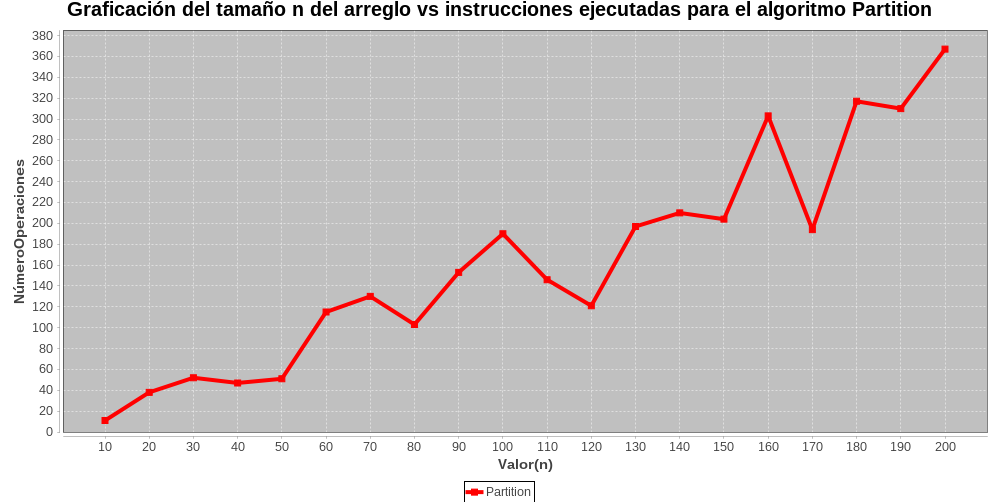
\includegraphics[width=13cm]{QuickSort/graf-partition.png}
            \caption{Representación gráfica de la complejidad temporal del algoritmo Partition, mediante la evaluación del número de instrucciones realizadas.}
            \label{GraficaPartition}
        \end{figure}
        
        \begin{figure}[h!]
            \centering
            \begin{tabular}{c|c}
                    P1( 10,11 ) & P11( 110,146 )\\
                    P2( 20,38 ) & P12( 120,121 )\\
                    P3( 30,52 ) & P13( 130,197 )\\
                    P4( 40,47 ) & P14( 140,210 )\\
                    P5( 50,51 ) & P15( 150,204 )\\
                    P6( 60,115 ) & P16( 160,303 )\\
                    P7( 70,130 ) & P17( 170,194 )\\
                    P8( 80,103 ) & P18( 180,317 )\\
                    P9( 90,153 ) & P19( 190,310 )\\
                    P10( 100,190 ) & P20( 200,367 )\\
            \end{tabular}
            \caption{Pares obtenidos de la evaluación del algoritmo Partition}
            \label{PuntosPartition}
        \end{figure}
        
        La gráfica generada por estos pares se muestra en la figura \ref{GraficaPartition}. Podemos apreciar que existe una dispersión de puntos que al contrario del algoritmo Merge no forman un patrón claro de recta, sin embargo, por las posiciones de los puntos podemos notar que pueden quedar acotados por una función lineal. A continuación, en la figura \ref{GraficaDesmosPartition} se propone la recta $y=2x$ y se considera la ecuación que describe la complejidad conocida para el algoritmo Partition como $y=x$.
        
        \begin{figure}[h!]
            \centering
            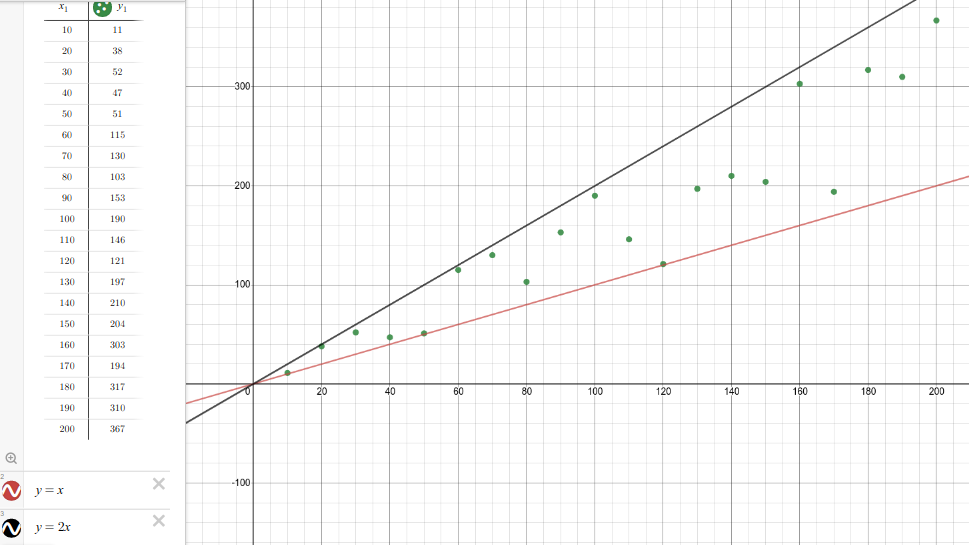
\includegraphics[width=13cm]{QuickSort/desmos-partition.png}
            \caption{Gráfica con función propuesta para acotar la complejidad de \textbf{Partition}. \\Los puntos verdes corresponden a los pares obtenidos en la evaluación del algoritmo. La recta en color negro corresponde a la ecuación conocida que describe la complejidad para el algoritmo \textbf{Partition}. La recta en color rojo corresponde a la cota propuesta para la complejidad de \textbf{Partition}.}
            \label{GraficaDesmosPartition}
        \end{figure}
        
        Para la eleccion de la constante multiplicativa de la cota propuesta en la figura \ref{GraficaDesmosPartition}, fue tomada al probar diversos valores y considerar que $y=2x$ era la que mejor se ajustaba en nuestro caso.
        
        
    \subsection*{Complejidad de \textbf{Partition} analíticamente}
        Para el cálculo analitico de la complejidad, retomaremos el pseudocódigo descrito en la figura \ref{PseudocodigoPartition}.
        
        \begin{equation*}
            \left.
                \begin{aligned}
                    \left.
                        \begin{aligned}
                            \text{pivote = A[ult]} \\
                            \text{i = prim-1} \\
                        \end{aligned}   
                    \right\}
                    \quad\Theta(1)
                    \\
                    \left.
                        \begin{aligned}
                            \text{for j=prim to j}<\text{ult do} \\
                            \text{if A[j]}<\text{pivote} \\
                            \text{int tmp=A[i]} \\
                            \text{A[i]=A[j]} \\
                            \text{A[j]=tmp} \\
                        \end{aligned}
                    \right\}
                    \quad\Theta(n)
                    \\
                    \left.
                        \begin{aligned}
                            \text{int tmp=A[i+1]} \\
                            \text{A[i+1]=A[ult]} \\
                            \text{A[ult]=tmp} \\
                            \text{return i+1} \\
                        \end{aligned}
                    \right\}
                    \quad\Theta(1)
                \end{aligned}
            \right\}
            \quad\Theta(n)
        \end{equation*}
        En el primer bloque encontramos una complejidad $\Theta(1)$ debido a que únicamente encontramos asignaciones a variables. Posteriormente, encontramos la complejidad del siguiente bloque que es $\Theta(n)$ que corresponde al bloque definido por el ciclo for que posiciona el pivote en el lugar correcto dentro del arreglo. Finalmente, el último bloque tiene una complejidad constante $\Theta(1)$ debido a que únicamente se ejecutan instrucciones que no pertenecen a ningún ciclo. Finalmente, se concluye que el algoritmo Partition posee una complejidad temporal lineal definida por $\Theta(n)$.
        
    \subsection*{Complejidad de \textbf{QuickSort} mediante gráficas}
        Para la generación de nuestras gráficas, se realizó un conteo del número de operaciones realizadas en el algoritmo por cada entrada de arreglo de tamaño n. Se utilizaron arreglos generados aleatoriamente con valores entre el 0 y el 9. EL tamaño del arreglo de entrada se modifica con la intención de obtener puntos graficables. Los puntos se muestran en la figura \ref{PuntosQSort}.\\
        
        \begin{figure}[h!]
            \centering
            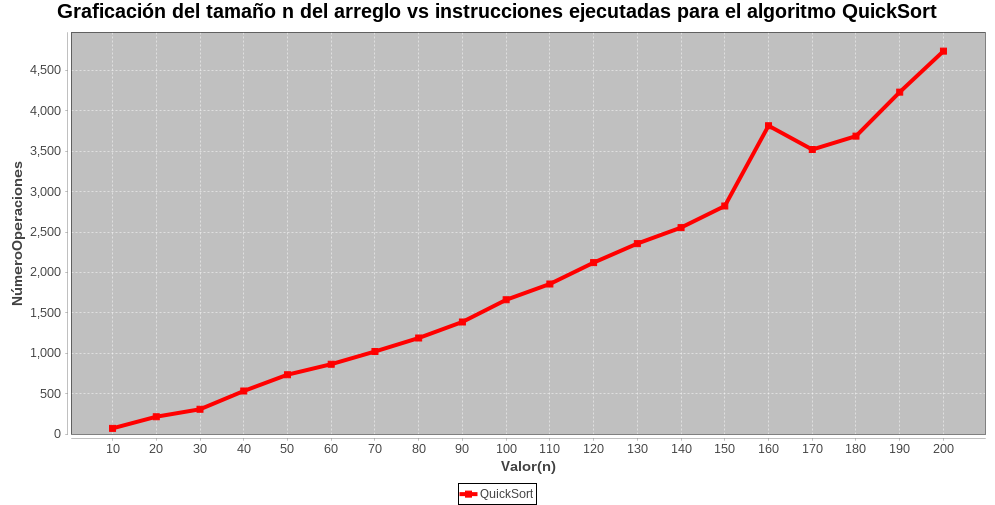
\includegraphics[width=13cm]{QuickSort/graf-qsort.png}
            \caption{Representación gráfica de la complejidad temporal del algoritmo \textbf{QuickSort}, mediante la evaluación del número de instrucciones realizadas.}
            \label{GraficaQSort}
        \end{figure}
        
        \begin{figure}[h!]
            \centering
            \begin{tabular}{c|c}
                    P1( 10,70 ) & P11( 110,1857 )\\
                    P2( 20,214 ) & P12( 120,2121 )\\
                    P3( 30,306 ) & P13( 130,2357 )\\
                    P4( 40,532 ) & P14( 140,2555 )\\
                    P5( 50,734 ) & P15( 150,2822 )\\
                    P6( 60,864 ) & P16( 160,3816 )\\
                    P7( 70,1021 ) & P17( 170,3521 )\\
                    P8( 80,1188 ) & P18( 180,3687 )\\
                    P9( 90,1387 ) & P19( 190,4232 )\\
                    P10( 100,1661 ) & P20( 200,4739 )\\
            \end{tabular}
            \caption{Pares obtenidos de la evaluación del algoritmo \textbf{QuickSort}}
            \label{PuntosQSort}
        \end{figure}
        
        La gráfica generada por estos pares se muestra en la figura \ref{GraficaQSort}. Es posible observar que el algoritmo muestra un ligero  patrón cuadrático de crecimiento. Debemos recordar que la funcion \textbf{Partition} divide al arreglo en dos subarreglos, sin embargo, no tenemos control del valor del pivote tomado por \textbf{Partition}.
        
        \begin{figure}[h!]
            \centering
            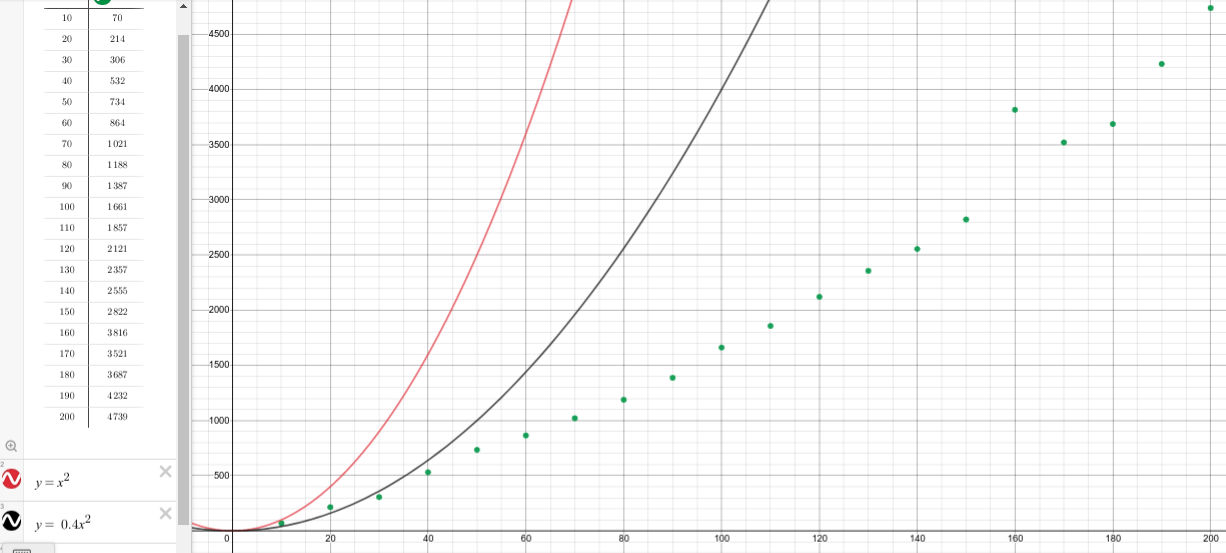
\includegraphics[width=17.5cm]{QuickSort/desmos-QSort.png}
            \caption{Gráfica con función propuesta para acotar la complejidad de \textbf{QuickSort}. \\Los puntos verdes corresponden a los pares obtenidos en la evaluación del algoritmo. La recta en color rojo $y=x^{2}$ corresponde a la ecuación conocida que describe la complejidad para el algoritmo \textbf{QuickSort}. La recta en color negro $y=0.4x^{2}$ corresponde a la cota propuesta para la complejidad de \textbf{QuickSort}.}
            \label{GraficaDesmosQSort}
        \end{figure}
        
        En la figura \ref{GraficaDesmosQSort} se propone como cota para el algoritmo a $y=x^{2}$ de acuerdo a los pares ordenados que se obtuvieron en la evaluación, 
        
    \subsection*{Complejidad de \textbf{QuickSort} analíticamente}
        Para el cálculo de la complejidad del algoritmo QuickSort consideraremos su pseudocódigo descrito en la figura \ref{PseudocodigoQSort}.
        
        \begin{figure}[h!]
        \centering
        \begin{verbatim}
            int[] QuickSort(A[], int prim, int ult)
                if prim < ult
                    int p = Partition(A, prim, ult)
                    QuickSort(A, prim, p-1)
                    QuickSort(A, p+1, ult)
                return A
        \end{verbatim}
        \caption{Pseudocódigo de la función QuickSort}
        \label{PseudocodigoQSort}
        \end{figure}
        
        Cuando el pivote divide el arreglo por la mitad, encontramos el mejor caso para el algoritmo QuickSort.
        
        \begin{equation*}
            \left.
                \begin{aligned}
                    \left.
                        \begin{aligned}
                            \text{q=Partition(A, prim, ult)}
                        \end{aligned}
                    \right\}
                    \quad\Theta(n)
                    \\
                    \left.
                        \begin{aligned}
                            \text{QuickSort(A, prim, q-1)}
                        \end{aligned}
                    \right\}
                    \quad T(q)
                    \\
                    \left.
                        \begin{aligned}
                            \text{QuickSort(A, q+1, n)}
                        \end{aligned}
                    \right\}
                    \quad T(n-q)
                    \\
                \end{aligned}
            \right\}
            \quad T(n) = T(q) + T(n-q) + \Theta(n)
        \end{equation*}
        
        De tal forma, se considerara \textbf{q=$\frac{n}{2}$}, y sustituimos en la ecuación de recurrencia:
        $T(n) = T(q)+T(n-q)+\Theta(n) \text{ Donde \textbf{q}, es la posición del pivote en el arreglo}$
                
        \begin{equation*}
            T(n)=T\left(\frac{n}{2}\right)+T\left(n-\frac{n}{2}\right)+\Theta(n) =2T\left(\frac{n}{2}\right)+\Theta(n)
        \end{equation*}
            
        Identificamos los elementos de la ecuacion:\\
        $a=2$\\
        $b=2$\\
        $f(n)=\Theta(n) = cn$\\
        Y procedemos a evaluar los requisitos del problema maestro:
        \begin{equation*}
            n^{log_ba}=n^{log2}=n
        \end{equation*}
        Se verifica entonces con respecto a \textbf{f(n)}:
        \begin{equation*}
            n=n^{log_ba}=f(n)=n
        \end{equation*}
            
        Por lo tanto, mediante el caso \textbf{II} del teorema maestro:
        \begin{equation*}
            T(n) = \Theta (n^{log_ba}logn) = \Theta(nlogn)
        \end{equation*}
        
    \subsection*{Proposición de orden de complejidad para \textbf{QuickSort} cuando todos los elementos del arreglo son distintos y están ordenados en forma decreciente.}
        
        En la figura \ref{GraficaQSortOrdenados} podemos observar el comportamiento del algoritmo teniendo como entrada un arreglo con todos los elementos distintos y ordenados de forma decreciente, para la generación de la gráfica consideramos el conteo de instrucciones ejecutadas.
        
        \begin{figure}[h!]
            \centering
            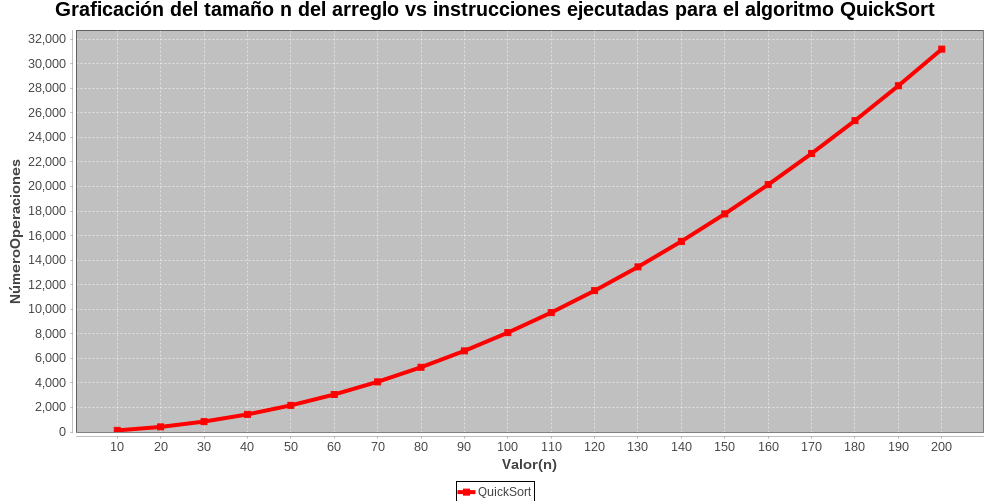
\includegraphics[width=13cm]{QuickSort/graf-qsort-ordenados.png}
            \caption{Representación gráfica de la complejidad temporal del algoritmo \textbf{QuickSort}, mediante la evaluación del número de instrucciones realizadas.}
            \label{GraficaQSortOrdenados}
        \end{figure}
        
        \begin{figure}[h!]
            \centering
            \begin{tabular}{c|c}
                    P1( 10,129 ) & P11( 110,9729 )\\
                    P2( 20,414 ) & P12( 120,11514 )\\
                    P3( 30,849 ) & P13( 130,13449 )\\
                    P4( 40,1434 ) & P14( 140,15534 )\\
                    P5( 50,2169 ) & P15( 150,17799 )\\
                    P6( 60,3054 ) & P16( 160,20154 )\\
                    P7( 70,4089 ) & P17( 170,22689 )\\
                    P8( 80,5274 ) & P18( 180,25374 )\\
                    P9( 90,6609 ) & P19( 190,28209 )\\
                    P10( 100,8094 ) & P20( 200,31194 )\\
            \end{tabular}
            \caption{Pares obtenidos de la evaluación del algoritmo \textbf{QuickSort} para el caso en que los elementos del arreglo son distintos y están ordenados de forma descendente.}
            \label{PuntosQSort}
        \end{figure}
        
        \begin{figure}[h!]
            \centering
            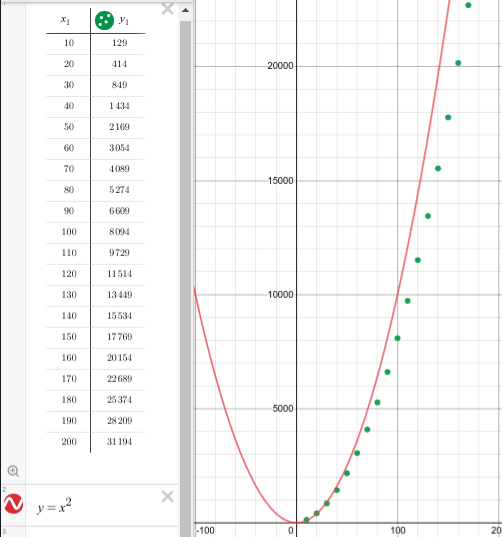
\includegraphics[width=13cm]{QuickSort/desmos-qsort-ordenado.png}
            \caption{Gráfica con función propuesta para acotar la complejidad de \textbf{Quicksort}. \\Los puntos verdes corresponden a los pares obtenidos en la evaluación del algoritmo. La función roja, es nuestra propuesta de cota superior para la complejidad temporal para el algoritmo Quicksort en su peor caso.}
            \label{GraficaDesmosPartition}
        \end{figure}
        
        Finalmente, podemos concluir que hemos comprobado gracias a nuestro analisis a posteriori, que el algoritmo posee una complejidad cuadrática para su peor caso.
        
